\documentclass[../../main.tex]{subfiles}

\begin{document}
\chapter{Contemporary Research}
Even though Marcus published his book in 2001, he still maintains his main points of criticism regarding popular connectionist models. In his blog posts he discusses contemporary research, and he points out fundamental weaknesses of popular connectionist models, including LLMs.

\begin{citecallout}[\textcite{marcus_black_box}]
    LLM are giant, opaque black boxes with no explicit models of the world at all. Part of what it means to say that an LLM is a black box is to say that you can’t point to an articulated model of any particular set of facts inside.
\end{citecallout}

\begin{citecallout}[\textcite{marcus_black_box}]
    But the LLM doesn't maintain structured symbolic systems like databases; it has no direct database of cities and populations. Aside from what it can retrieve with external tools like web searches (which provide a partial but only partial workaround) it just has a bunch of bits of text that it stochastically reconstructs. And that is why they hallucinate, frequently. They wouldn't need to do so if they actually had reliable access to relevant databases.
\end{citecallout}

\section{The Illusion of Thinking}
In order to improve the symbolic capabilities of LLMs, researchers suggested various methods, including \emph{Large Reasoning Models} (LRMs). \textcite{illusion-of-thinking} acknowledge this in their paper \emph{The Illusion of Thinking}:

\begin{newcite}[\textcite{illusion-of-thinking}]
    While these LLMs demonstrate promising
    language understanding with strong compression capabilities, their intelligence and reasoning abilities
    remain a critical topic of scientific debate [7, 8]. Earlier iterations of LLMs [ 9, 10, 11] exhibited
    poor performance on reasoning benchmarks [12, 13, 14, 6]. To address these shortcomings, several
    approaches have been explored with the common theme among them being “scaling” both the training
    data and test-time computation. For instance, generating a Chain of Thought (CoT) [15, 16, 17, 18]
    and incorporating self-verification [19, 20, 21] prior to the final answer have been shown to improve
    model performance.
\end{newcite}


The authors of this paper analyzed how well standard LLMs could solve classical search problems like \emph{The Tower of Hanoi}, and to what extend LRMs improve symbolic capabilities. They tested several models on varying problem complexities, like different number of starting disks in the case of Tower of Hanoi.

What they found is that both LLMs and LRMs have high accuracy on simple problems. As complexity increases, reasoning models outperform their non-reasoning counterparts, until both reach a point where the models are unable to solve the problem at all. These findings are summarized in figure~\ref{fig:illusion-of-thinking}.

\begin{figure}[htbp]
    \centering
    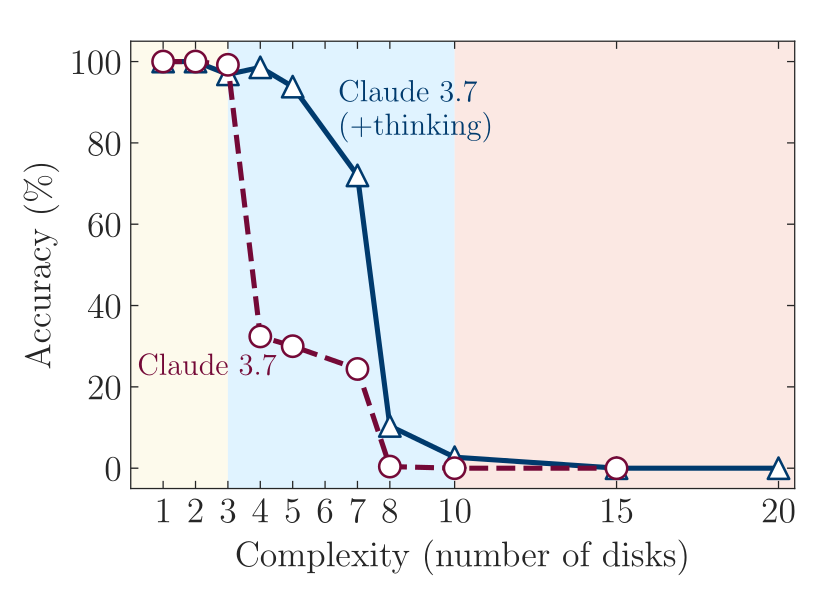
\includegraphics[width=0.8\textwidth]{./chapters/contemporary_research/accuracy_at_complexity.png}
    \caption{Performance of LLMs and LRMs on Tower of Hanoi problems with varying complexity. Source: \textcite{illusion-of-thinking}.}
    \label{fig:illusion-of-thinking}
\end{figure}

Other conclusions of the paper are:

\begin{newcite}[\textcite{illusion-of-thinking}]
    Our detailed analysis of reasoning traces further exposed complexity-dependent reasoning patterns, from inefficient “overthinking” on simpler problems to complete failure
    on complex ones. These insights challenge prevailing assumptions about LRM capabilities and
    suggest that current approaches may be encountering fundamental barriers to generalizable reasoning.
    Finally, we presented some surprising results on LRMs that lead to several open questions for future
    work. Most notably, we observed their limitations in performing exact computation; for example,
    when we provided the solution algorithm for the Tower of Hanoi to the models, their performance
    on this puzzle did not improve. Moreover, investigating the first failure move of the models revealed
    surprising behaviors. For instance, they could perform up to 100 correct moves in the Tower of
    Hanoi but fail to provide more than 5 correct moves in the River Crossing puzzle.
\end{newcite}

Marcus argues that this paper provides evidence for his claim of poor symbolic capabilities of connectionist models due to insufficient \emph{structured symbolic systems}:

\begin{citecallout}[\textcite{marcus_knockout_blow}]
    The new Apple paper adds to the force of Rao's critique (and my own) by showing that even the latest of these new-fangled “reasoning models” still—even having scaled beyond o1—fail to reason beyond the distribution reliably, on a whole bunch of classic problems, like the Tower of Hanoi. For anyone hoping that “reasoning” or “inference time compute” would get LLMs back on track, and take away the pain of m multiple failures at getting pure scaling to yield something worthy of the name GPT-5, this is bad news.
\end{citecallout}

\begin{critique}
    While the findings of \textcite{illusion-of-thinking} are compelling, their methodology warrants critical examination. As the authors themselves acknowledge, the reliance on highly algorithmic tasks like the Tower of Hanoi may not be representative of all forms of reasoning. Furthermore, given the known sensitivity of LLMs to prompt phrasing, it remains an open question whether the observed performance limits are fundamental to the models themselves or an artifact of the specific prompting strategies employed.

    Additionally, Marcus's conclusion that these shortcomings prove the models are incapable of reasoning is too strong. The paper itself shows that the models have better reasoning capabilities on problems that are more popular, suggesting performance is heavily influenced by representation in the training data. While an untrained model clearly lacks reasoning abilities, these skills demonstrably improve with training. Therefore, one cannot rule out the possibility that with sufficient scale and the right data, these models could eventually meet the demands of complex symbolic tasks.
\end{critique}

\section{A Case for Neuro-Symbolic AI: AlphaGeometry}
After having analyzed Marcus's critique of purely connectionist models, it seems less surprising that he is an advocate of \emph{neuro-symbolic AI}, which integrates neural and symbolic AI architectures to address the weaknesses of each. Marcus writes in his article \citetitle{marcus_alphageometry}:

\begin{citecallout}[\textcite{marcus_alphageometry}]
    The idea is to try to take the best of two worlds, combining (akin to Kahneman's System I and System II), neural networks, which are good at kind of quick intuition from familiar examples (a la Kahneman's System I) with explicit symbolic systems that use formal logic and other reasoning tools (a la Kahneman's System II).
\end{citecallout}

One of these hybrid models is Google's \emph{alphageometry}, which the authors described in \citetitle{Trinh2024}. Amongst all the hype around connectionist models, Marcus highly values this paper:

\begin{citecallout}[\textcite{marcus_alphageometry}]
    Which brings me to one of the few AI reports I have liked lately, their blog this week on progress on the International Math Olympiad, in which (with some caveats) they achieved Silver Medal performance, far ahead of what most humans could manage.
\end{citecallout}

In order to understand the claimed interplay of connectionism and symbolism, we have to take a closer look at the paper. These are the results in a nutshell according to the authors:

\begin{newcite}[\textcite{Trinh2024}]
    AlphaGeometry is a neuro-symbolic system that uses a neural language model,
    trained from scratch on our large-scale synthetic data, to guide a symbolic deduction
    engine through infinite branching points in challenging problems. On a test set of
    30 latest olympiad-level problems, AlphaGeometry solves 25, outperforming the
    previous best method that only solves ten problems and approaching the performance
    of an average International Mathematical Olympiad (IMO) gold medallist.
\end{newcite}

\begin{figure}[htbp]
    \centering
    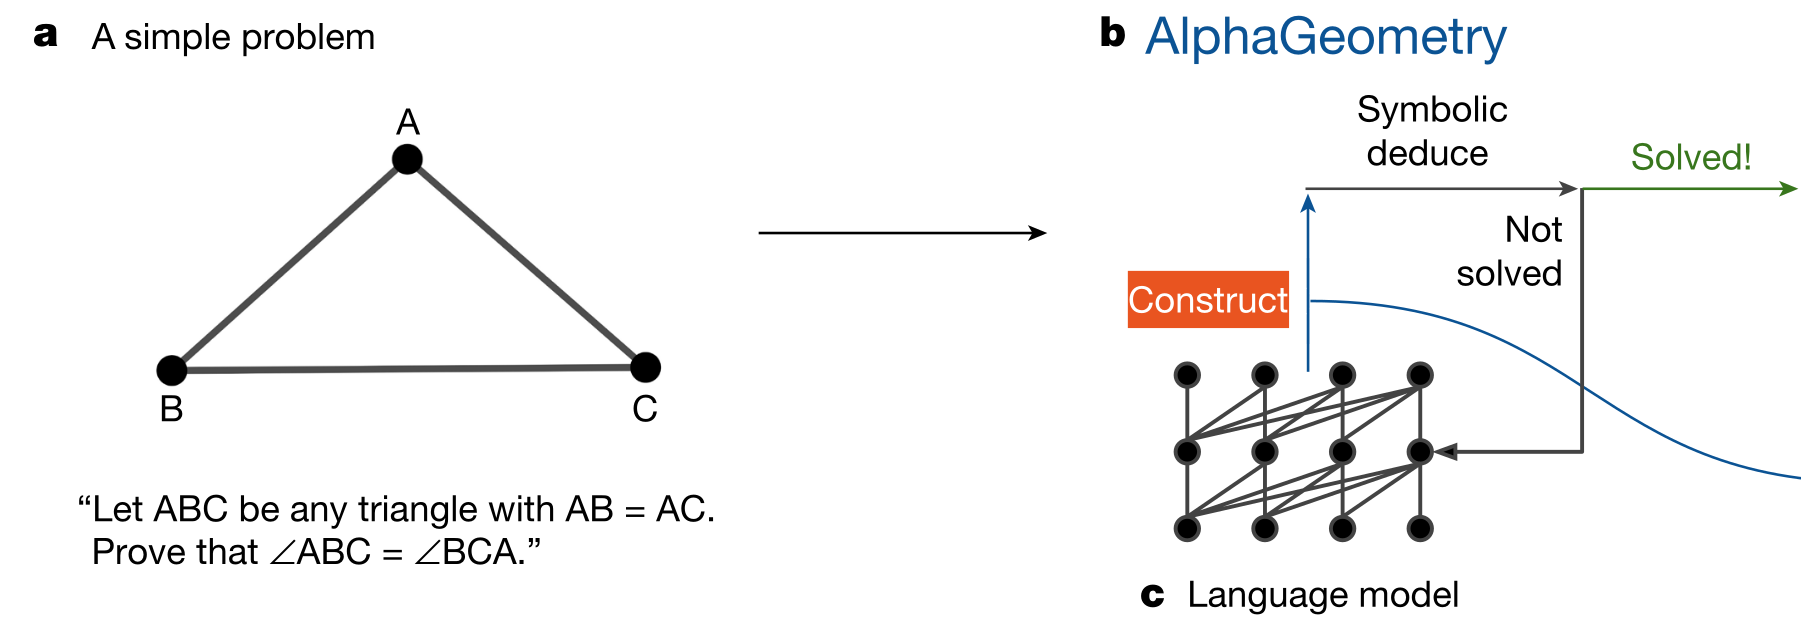
\includegraphics[width=0.8\textwidth]{chapters/contemporary_research/alphageometry.png}
    \caption{Overview of the neuro-symbolic AlphaGeometry model. \\ Source: \textcite{Trinh2024}}
    \label{fig:alphageometry}
\end{figure}

One can think of the model this way: The deduction engine explores a search graph, where it is given the starting point, that is the premises of the problem, and the endpoint, that is the theorem to prove. Based on \emph{deductive database}, the symbolic engine can explore paths in this network. However, since some problems require additional assumptions to be made, like defining new points, an exhaustive search may not always yield the answer right away.

This is where language model comes in. It tries to predict the necessary steps needed to take in the proof, where its intuition serves to create new premises. This information is then fed back into the deduction engine. This cycle continues until the engine infers the desired statement of interest, or until a timeout occurs.

\bigskip
In the same blog post where Marcus discusses these advancements, he concludes:

\begin{citecallout}[\textcite{marcus_alphageometry}]
    There can be no path to AGI without neurosymbolic AI.
\end{citecallout}

This conclusion is the result of his persistent critique on purely connectionist models, as well as results like AlphaGeometry which mark great advancements in AI and are based on neuro-symbolic architectures.

\chapter{Summary}
For over two decades, Gary Marcus has established himself as a prominent and persistent critic of purely connectionist approaches to artificial intelligence. His 2001 book, The Algebraic Mind, laid the foundation for his main line of argumentation: that connectionist models, on their own, lack the necessary architecture for true generalization and the kind of systematic, algebraic reasoning that is central to human cognition.

As this analysis has shown, Marcus's specific frameworks—such as his reduction of algebraic rules to UQOTOMs—and the formal structure of his arguments can be challenged for their simplicity and speculative nature. His proposed solutions, like a register-based architecture, often lack the concrete, testable detail he demands of the models he critiques.

Despite these methodological weaknesses, his core message should not be overlooked. Marcus’s fundamental critique—that a field focused solely on one paradigm risks ignoring essential components of intelligence—remains highly relevant. Even today, he actively engages with contemporary research, interpreting findings from papers on both the limitations of LLMs and the successes of neuro-symbolic systems like AlphaGeometry as further evidence for his long-standing claims.

Now that we have presented Marcus's views, the empirical evidence he draws upon, and the critiques of his own framework, it is up to the reader to decide on which points they agree with Marcus or where the weaknesses in his arguments lie. We hope to have illuminated this important debate from multiple viewpoints, so that the reader may form their own critical opinion.
\end{document}